\section{P2Pedia, a P2P Wiki}
\label{sec:proposal}
\subsection{Functional Overview}
P2Pedia, our Wiki system, is accessed through a web browser, and its interface is similar to that of most existing Web-based Wikis. Users may browse pages, perform keyword searches (on the page title and/or on the textual content), and edit any page, as in a traditional wiki, by clicking on a tab at the top of the page, and editing Wikitext in a text box, using the Creole Wiki Syntax \cite{creole1.0spec}. 

A screenshot of the P2Pedia interface, where a document is being edited, is shown in Figure \ref{fig:screenshot}.

\begin{figure*}[tb]
\centering
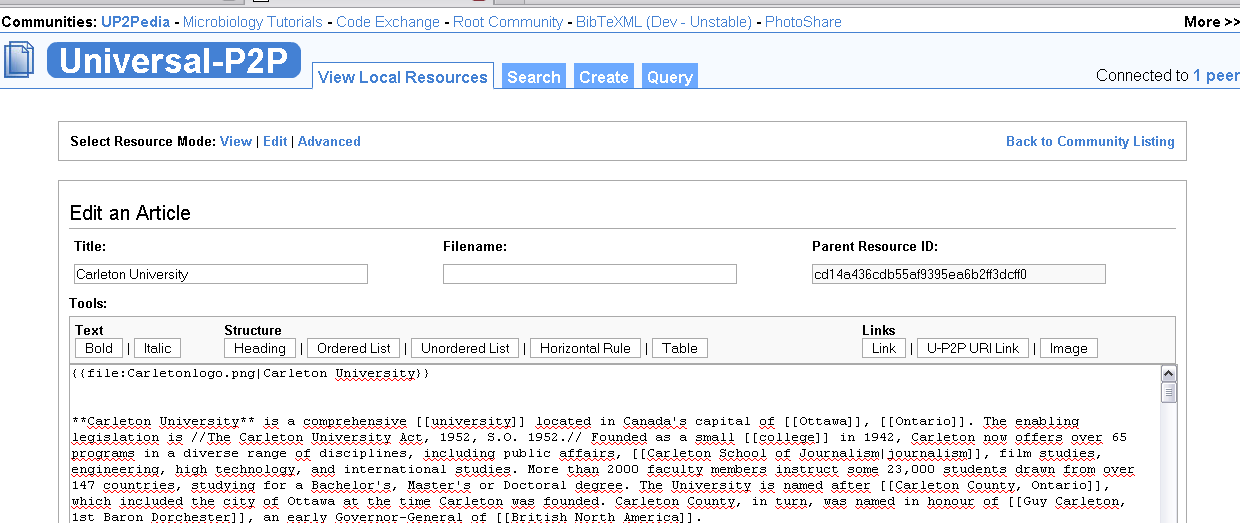
\includegraphics[scale=0.4]{screenshot.png}
\label{fig:screenshot}
\caption{A screenshot of the P2Pedia interface. The user is editing a page.}
\end{figure*}


The main difference with a traditional wiki is that as pages are downloaded to be viewed, they are also saved locally, and an edit creates a new version of the document, which is also stored locally. Therefore, as an article is edited, it may be ``forked" into multiple versions, and each peer is free to save and offer for download its preferred version. 

If a user searches for a page, different versions may be returned by different peers. The user may then use the versioning relationships between these versions, and trust indicators (detailed in section \ref{sec:trust}) about the documents and the peers, to decide which version to download. 

As multiple parallel versions may exist, users may also produce new versions by \emph{merging} several existing versions, selecting and reusing different parts of several \emph{parent} versions, and producing a single \emph{child} version. 

\subsection{Wiki Edition as an Application of File-sharing}

P2P File-sharing, mostly known as an application to share media files, can be applied to other types of content. Here, we show how the functionality of a distributed wiki can be mapped to an abstract model of file-sharing. We have used this mapping as a basis to implement P2Pedia on top of U-P2P, our file-sharing application \cite{UP2P2002, UP2PSemelsJournal2009, UP2P:201101TechReport}.

We first outline our model of file-sharing, implemented by U-P2P and more completely presented in \cite{UP2P:201101TechReport}. P2P file-sharing can be characterized as an application where peers, connected in a network, maintain a collection of \emph{documents} in a local repository. Peers may publish new documents to the repository, remove them, or copy (i.e. download) documents from other peers.

Peers can join or leave the network, and establish or drop connections with other peers. These operations define possible \emph{state changes} for the network. 

We then introduce the concept of a \emph{community}. A community is defined by a document \emph{schema} and a protocol (means for queries to reach peers). The schema is a set of attributes, and defines the type of documents that are shared in the community (music, video, or any other kind). consequently, it also defines which queries may be applied to these documents. 

This model can describe traditional file-sharing applications such as Limewire\footnote{official web site is http://www.limewire.com/, distribution currently suspended.} or Emule\footnote{http://www.emule-project.net/}. For example, Limewire can be defined as a community where MP3 music files are shared using the Gnutella 0.6 protocol with a TTL (time to live) of 7. The documents of this community are described by a file name, a binary ``payload", and a set of metadata properties, encoded in ``ID3 tags"\footnote{``ID3 tags" are data fields embedded into MP3 files, which identify the artist, song title, track number, etc.}. A peer may then communicate with all the peers reachable by a path of length of at most seven hops (seven edges in the connection graph), and can make queries on the file name, or on any of the ID3 metadata properties. 

An important feature of U-P2P is that community definitions can themselves be shared in the P2P network. This way, peers can create new such communities, and discover and download those created by others. A community description includes a document schema, which itself can be used as a guide for metadata-based searches.

We have further extended this model to include \emph{relations} between documents. Such relations are irrelevant to basic applications where ordinary media files are shared, but are useful for other types of documents, for example Wiki pages, which can be related by versioning relations and wikilinks.

For this purpose we have added a type of document attribute, called \emph{endpoints}, similar to web links. Endpoints rely on a naming scheme (i.e. a ``primary key" that unambiguously identifies any document), and represent a semantic link to that document, this semantics being carried by the attribute label. For example, our wiki pages refer to their \emph{parent} documents using such links. 

In addition to the semantics represented by the attribute label, an important difference with Web links is that endpoints, in a P2P file-sharing context, must point to \emph{any copy} of the target document, which may be replicated through the network. Looking up a document given its endpoint therefore means searching for all copies of the document by that unique name. The document naming scheme is therefore based on the document content rather than on an address. In practice, document identifiers in U-P2P are generated by a one-way hash function.

Graph queries can then be applied to the graph of documents (nodes), connected by endpoint attributes (edges) \cite{UP2P:201101TechReport}. 

Here, P2Pedia defines a community, where each shared file is a Wiki page. The document schema includes the page content (the wikitext), the versioning information, in the form of a multi-valued endpoint attribute to parent versions, and a number of wikilinks to other pages. The wiki engine is then simply a tool -- two small Javascript scripts -- provided as part of the community definition, for viewing and editing documents of the community.

The main functionality of the system is implemented by the standard file-sharing operations, namely publish, remove, query, and download. Searches for pages are implemented as file-sharing queries, and users download pages from other peers, just like any document in a file-sharing network. When peers edit pages, they create a new document, which links back to its parent documents using an endpoint attribute.

An endpoint attribute, as a link between two documents, can be viewed as a binary relation over the set of documents. The properties of the relations in P2Pedia (i.e. associated to the endpoint attributes of the P2Pedia schema) give a greater semantic interpretation to the graph queries made over  the P2Pedia document graph. In the next section, we define these semantic properties, and then show how appropriate queries over the graph of documents can be used to implement useful functionality for P2Pedia.

\subsection{Ancestry Relations, and the Semantics of Wikilinks}
\label{sec:ancestry}
The versioning process can be characterized by the properties of the \emph{parent} and \emph{child} binary relations between documents, and their respective transitive closures \emph{ancestor} and \emph{descendent}. 

The centralized collaboration model, implemented by traditional wikis, produces a linear versioning process, where the latest version is considered ``authoritative". If we consider each version of a page to be a separate document, a sequence of page versions is a set of documents, which all have the same page title, and the \emph{``child"} relation defines a total order over this set. This order is the order of the timestamps of the different versions. 

Wikilinks consequently have a clear semantics: a wikilink is defined by its \emph{label}, and points to the latest version of the page with that label for a title, i.e., within the set of page versions defined by that label, to the upper bound in the sense of the \emph{child} relation. 

In contrast, as we have mentioned above, the versioning process offered by our collaboration model produces a \emph{lattice} of versions for each page, where a given document version may have multiple \emph{children} versions (edits) and multiple \emph{parent} versions. Page titles and timestamps are then insufficient indicators of the version relationships between pages: the \emph{parent} and \emph{child} relation must be explicit within the pages, and define only a partial order over set of versions of a page with a given title. Figure \ref{fig:versioninglattice} shows this lattice versioning hierarchy compared with the sequential hierarchy produced by a centralized collaboration model (Figure \ref{fig:versioningsequence}). 

\begin{figure}[htb]
\centering
\subfigure[Versioning in a centralized Wiki: v3 is the ``current" version.]{
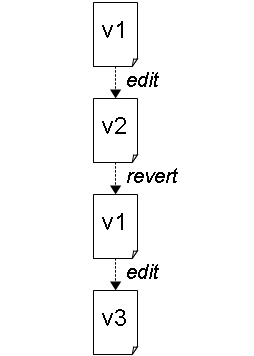
\includegraphics[scale=0.44]{versioning-sequence.png}
\label{fig:versioningsequence}
}
\subfigure[Versioning in P2Pedia: v5 and v6 are ``maximal" versions in the versioning lattice.]{
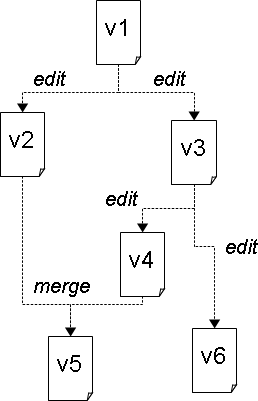
\includegraphics[scale=0.56]{versioning-lattice.png}
\label{fig:versioninglattice}
}
\caption{The different versioning processes available in a centralized and decentralized collaboration model produce different versioning hierarchy structures. Each figure shows an example hierarchy of versions for a single page.}
\end{figure}

Extending the notion of a wikilink to a set of page versions with a lattice structure is not trivial. In the linear case, there is always a single latest version, and we can therefore relate the document that the user originally linked to, with its unique last descendent, the current latest version. In the lattice case, there may be at any given time multiple ``latest" versions, and a user could intend to link to any one of these versions. Furthermore, from the originally linked version, there may be an entire tree of descendents, and any leaf of this tree would be a candidate to be the ``current version". 

This shows two requirements for wikilinks in this collaboration model. First, when creating a wikilink, a user should be able to explicitly choose any particular version of a page as the target. Secondly, the wikilink should link to multiple pages, i.e. it the link should return all the leaf-descendants of the originally linked document. 

Formally, this means that the binary relation defined by a wikilink defined within a document $A$, and originally pointing to document $B_0$, contains all pairs $(A, B_i)$ where $A$ is the document containing the link, and $B_i$ is a leaf-descendant of $B$.

The decentralized storage of our system further complicates the nature of the ancestry relation. As documents are copied through the network, the ``parent" links point to \emph{all copies} of the parent document version. The versioning process in Figure \ref{fig:versioninglattice}, combined with some downloads, could result in a distributed graph such as the one illustrated in Figure \ref{fig:versioning-deploy}. 

\begin{figure}[htb]
\centering
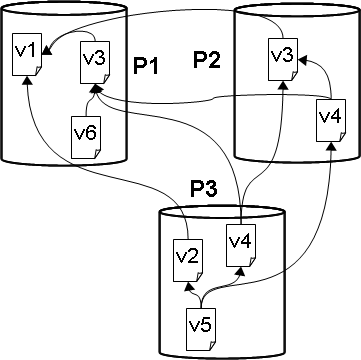
\includegraphics[scale=0.5]{doc-links-deploy.png}
\label{fig:versioning-deploy}
\caption{An example deployment of the document versions shown in Figure \ref{fig:versioninglattice}. The documents are distributed in three peers P1, P2, P3. The arrows represent ``parent" links between document versions.}
\end{figure}

A user may maintain a version that she consider ``authoritative", and if another peer has copied and edited this version, it is no longer a ``leaf" (maximal element) in the lattice of versions. Therefore in the above discussion, the leaves in the tree of descendents for a particular document must include the latest version stored by each peer, regardless of whether these version have been edited elsewhere.

In practice, this means that a wikilink is implemented as a search for all the descendents of the document that this link originally pointed to, and each peer returns its latest version. The search for the descendents of a page can be implemented by a generic U-P2P graph query that returns the transitive closure of the ``child" relation. The ``child" relation is not itself explicit in U-P2P, but its inverse relation ``parent" is implemented as an endpoint attribute, and can therefore be exploited by graph queries in U-P2P.

The class of graph queries supported by U-P2P \cite{UP2P:201101TechReport}, \emph{path queries}, are defined as follows. In the graph of interlinked documents, where documents are nodes and endpoint attributes are labeled edges, a path query can be defined by an input document $D$ and a sequence of labels $\pi = l_1,l_2 \dots, l_k$; an answer to this query is a document $A$ such that the edge labels on the path from $D$ to $A$ match $\pi$. The endpoint attributes are seen as directed edges, but queries can be defined for paths including the edges in both directions (i.e. both properties explicited by links and their implicit inverses can be queried, for example if the relation ``parent" is explicited by a link, then the relation ``child" can also be queried).

For P2Pedia we have extended this class of queries to include \emph{transitive closure} queries. This means that we can query for paths matching a particular sequence of symbols $l_1,l_2 \dots, l_k$, but also for paths matching the regular expression $l_0^{+}$.

P2Pedia supports queries for the transitive closure of ``parent" and its inverse, ``child", the latter being used to resolve wikilinks.

These queries return multiple documents, as do simple keyword searches. The user must then be assisted in choosing between them. For this purpose we introduce trust indicators, detailed in the next subsection. Note that in any search, the relevance to the query, as well as the visible ancestry of the versions, can be used to choose. However, in all cases, additional trust information may be useful. 

\subsection{Trust Indicators}
\label{sec:trust}

Traditional wikis often limit which users may contribute, or resolve conflicts as they occur, by attempting to determine (by a consensus, or by other decision processes), which single version of an document should be accepted. These principles can be described as centralized trust strategies, i.e. where the ``trustworthiness" of the contributors is a unique value determined by the overall system.

The collaboration model of U-P2P allows for multiple versions of the articles, and therefore it allows for decentralized trust strategies, i.e. strategies where each user may have its own trust level toward each peer (multiple-authority).

In P2Pedia, trust levels are not explicitly maintained within the system, but each time a user must choose a document between several versions offered by different peers, she is provided some indicators which may help her determine which peers and documents are the most trustworthy.

The indicators implemented in P2Pedia are listed hereafter.

\paragraph*{Peer Similarity} A measure of similarity between the collections of documents hosted by the two peers (i.e. the peer who is viewing the query results, and the peer who offers a particular result). This indicator is based on the assumption that users storing similar content (i.e. a high number of identical versions of documents) should trust one another more. The indicator given is the Jaccard similarity measure, i.e. the number of document ids in common divided by the total number of documents stored by the two peers.
\paragraph*{Network Distance} This indicator shows the distance between the peers in the connection graph. Assuming that peers connect to trusted acquaintances, and that trust has some level of transitivity, the network distance may help the peer decide on trust.
\paragraph*{Peer Popularity} The number of incoming connections to a remote peer. Again, if peers connect to trusted acquaintances, or decide to connect to peers that offer high quality content, then the indegree of a peer in the connection graph is a valuable indicator of general trustworthiness.
\paragraph*{Document Popularity} The total number of available sources for a given version of a document. This assumes that the replication of documents is a measure of their ``value". 
    
Note that for a peer to be deemed trustworthy according to the above indicators and to fully be able to use them for its own benefit, it must actively maintain its content (by keeping documents that it ``endorses" and deleting the others) and its neighborhood (by connecting to similar peers and disconnecting from those that it doesn't trust anymore).     
